\section{Experimental Results}
\label{sec:results}

\subsection{Safety Performance}

Table~\ref{tab:cbf_violation_jpc} reports CBF constraint violation rates under $\Phi$-scaled nonlinear dynamics. The nominal HOCBF suffers $>95\%$ violation under all dynamics-affecting scenarios ($\Deltaf \neq 0$). GP mean correction alone (PPO-GP-HOCBF, $\epsilon=0$) reduces violation to 0\% under constant perturbations (S1, S2, S4--S6) but leaves $45.4\%$ violation under the state-dependent perturbation S3 (Coupled). Adding the compositional $\epsilon(x)$ (PPO-RHOCBF, $\epsilonKappa = 1.0$) achieves no observed CBF violations ($0/250$ episodes; 95\% episode-level Wilson upper bound $1.46\%$) across nominal operation and all six static perturbation scenarios. LQR+RHOCBF achieves identical safety, confirming that the safety guarantee comes from the filter rather than the policy class. NMPC achieves 0\% violation on constant perturbations via offset-free disturbance estimation but lacks a probabilistic safety certificate.

\begin{table}[htbp]
    \centering
    \caption{Constraint Violation Rate (\%) under $\Phi$-Scaled Nonlinear Dynamics (mean $\pm$ std over 5 seeds). 0\% rates: $0/250$ episodes, 95\% Wilson upper bound $1.46\%$.}
    \label{tab:cbf_violation_jpc}
    \footnotesize
    \begin{tabular}{lccccccc}
        \toprule
        Method & Nominal & S1 & S2 & S3 & S4 & S5 & S6 \\
        \midrule
        PPO-HOCBF & $0.0$ & $100.0$ & $99.9$ & $99.9$ & $99.9$ & $99.5$ & $99.9$ \\
        PPO-GP-HOCBF & $0.0$ & $0.0$ & $0.0$ & $45.4$ & $0.0$ & $0.0$ & $0.0$ \\
        \textbf{PPO-RHOCBF} & $\mathbf{0.0}$ & $\mathbf{0.0}$ & $\mathbf{0.0}$ & $\mathbf{0.0}$ & $\mathbf{0.0}$ & $\mathbf{0.0}$ & $\mathbf{0.0}$ \\
        LQR-RHOCBF & $0.0$ & $0.0$ & $0.0$ & $0.0$ & $0.0$ & $0.0$ & $0.0$ \\
        NMPC & $0.0$ & $0.0$ & $0.0$ & $0.0$ & $0.0$ & $0.0$ & $0.0$ \\
        \bottomrule
    \end{tabular}
\end{table}

\textbf{Selective vs.\ saturated QP intervention.} Table~\ref{tab:qp_intervention_jpc} shows that the QP intervention rate is proportional to the perturbation magnitude. At $10$--$15$\,kJ/kg enthalpy perturbation (Moderate/Mag10), the filter intervenes on only $3.5$--$9.8\%$ of steps---the policy produces safe actions on $>90\%$ of steps. At baseline S1 magnitude ($50$\,kJ/kg), intervention saturates at $100\%$, reflecting the severity of model mismatch. The filter solves a nearest-action projection (minimally invasive by construction); under severe mismatch, the robust constraint becomes active at nearly every step, consistent with the filter's role as the safety-certified component.

\begin{table}[htbp]
    \centering
    \caption{QP Intervention Rate (\%) vs.\ Perturbation Magnitude (PPO-RHOCBF, $\epsilonKappa=1.0$, 3 seeds).}
    \label{tab:qp_intervention_jpc}
    \begin{tabular}{lccccc}
        \toprule
        & Mag10 & Moderate & Mag25 & Mag50 (S1) & Mag75 \\
        $\Delta f_h$ (kJ/kg) & $-10$ & $-15$ & $-25$ & $-50$ & $-75$ \\
        \midrule
        CBF\% & $0.0$ & $0.0$ & $0.0$ & $0.0$ & $0.0$ \\
        QP\%  & $3.5$ & $9.8$ & $49.4$ & $99.9$ & $100.0$ \\
        \bottomrule
    \end{tabular}
\end{table}

\subsection{Time-Varying Disturbances}

Table~\ref{tab:timevarying_jpc} reports performance under time-varying disturbances not seen during training. NMPC degrades under fast-switching disturbances (TV3: $19.7\%$) because its EMA disturbance estimator cannot converge fast enough. The Robust HOCBF filter with fixed GP maintains significantly lower violation (TV3: $7.7\%$). A GP-augmented NMPC variant (simplified cautious MPC, GP mean replacing EMA; full $\sigma_{\mathrm{GP}}$ horizon propagation omitted) improves under slowly-varying disturbances (TV3: $12.3\%$ vs.\ $19.7\%$) but degrades dramatically under step disturbances (TV1/TV2: $49\%$/$49\%$) because the GP's smooth mean injects systematic bias at transition points. The Robust HOCBF filter avoids this by separating GP mean correction (CBF constraint) from prediction-model roll out. Robust HOCBF achieves comparable constraint satisfaction to NMPC under static perturbations, lower violation under fast time-varying disturbances, substantially lower online computation time, and a per-step high-probability safety certificate under the fixed-GP assumptions.

\begin{table}[htbp]
    \centering
    \caption{HOCBF Violation Rate (\%) under Time-Varying Disturbances (mean $\pm$ std over 20 episodes $\times$ 300 steps). NMPC std $=0$ reflects deterministic computation. TV1--TV3 denote time-varying disturbance shapes and are distinct from the static perturbation labels S1--S6 in Table~1. The NMPC+GP variant is a simplified cautious MPC (GP mean replacing EMA; full $\sigma_{\mathrm{GP}}$ horizon propagation omitted); it is not a full chance-constrained GP-MPC baseline.}
    \label{tab:timevarying_jpc}
    \begin{tabular}{lccc}
        \toprule
        Method & TV1: Step & TV2: Fast Step & TV3: Random Walk \\
        \midrule
        NMPC & $2.00 \pm 0.00$ & $5.00 \pm 0.00$ & $19.67 \pm 0.00$ \\
        NMPC+GP (simplified) & $49.00 \pm 0.00$ & $48.67 \pm 0.00$ & $12.33 \pm 0.00$ \\
        \textbf{PPO-RHOCBF (fixed GP)} & $\mathbf{1.75 \pm 0.85}$ & $\mathbf{1.58 \pm 0.84}$ & $7.73 \pm 0.73$ \\
        \bottomrule
    \end{tabular}
\end{table}

\subsection{Process Control Performance}

Table~\ref{tab:process_metrics} reports process control performance metrics under three representative perturbation scenarios (PPO-RHOCBF, $\epsilonKappa = 1.0$, 1 seed $\times$ 500 steps). The integral absolute error (IAE) quantifies tracking cost; the maximum deviation and constraint margin characterize worst-case excursions; the input variation measures control smoothness. The inter-sample violation rate is $0.0\%$ across all three scenarios (4 sub-steps per control interval, $T_s = 1$\,s), providing empirical evidence that no inter-sample violation occurs in the tested representative trajectories. We do not claim a formal discrete-time invariance theorem; the continuous-time certificate of Theorem~1 is the formal guarantee.

\begin{table}[htbp]
    \centering
    \caption{Representative process-control performance under $\Phi$-scaled nonlinear dynamics (PPO-RHOCBF, $\epsilonKappa=1.0$, single evaluation run, 500 steps). IAE = integral absolute error; MaxDev = maximum absolute deviation from reference; Margin = minimum constraint margin (positive = safe); Input var.\ = total input variation; Inter-sample = fraction of steps with inter-sample constraint violation (4 sub-steps).}
    \label{tab:process_metrics}
    \footnotesize
    \begin{tabular}{lccc}
        \toprule
        Metric & S1: Heat & S3: Coupled & S5: Valve \\
        \midrule
        IAE$_{\mathrm{pressure}}$ (MPa$\cdot$s)  & 2301 & 1971 & 1841 \\
        IAE$_{\mathrm{enthalpy}}$ (kJ/kg$\cdot$s) & 13076 & 13094 & 13108 \\
        IAE$_{\mathrm{power}}$ (MW$\cdot$s)       & 0.0 & 0.0 & 10000 \\
        MaxDev$_{\mathrm{pressure}}$ (MPa)        & 4.60 & 3.95 & 3.68 \\
        MaxDev$_{\mathrm{enthalpy}}$ (kJ/kg)      & 26.2 & 26.2 & 26.3 \\
        MaxDev$_{\mathrm{power}}$ (MW)            & 0.0 & 0.0 & 20.0 \\
        Min.\ constraint margin                   & 12.7 & 60.3 & 8.2 \\
        Input variation (total)                   & 0.7 & 1.2 & 0.4 \\
        QP intervention (\%)                       & 100.0 & 100.0 & 100.0 \\
        Inter-sample violation (\%)               & 0.0 & 0.0 & 0.0 \\
        \bottomrule
    \end{tabular}
\end{table}

Under severe model mismatch (S1--S5), the QP filter intervenes at every step, and the tracking error reflects the geometry of the QP feasible region contracted by $\epsilon(x)$. The minimum constraint margin remains positive (safe) across all scenarios, confirming that $\epsilon(x)$ provides a sufficient buffer. The inter-sample violation rate of $0.0\%$ validates the sampled-data implementation: at $T_s = 1$\,s, the zero-order hold does not induce constraint violations between samples.

\subsection{Computational Efficiency}

\begin{figure*}[t]
    \centering
    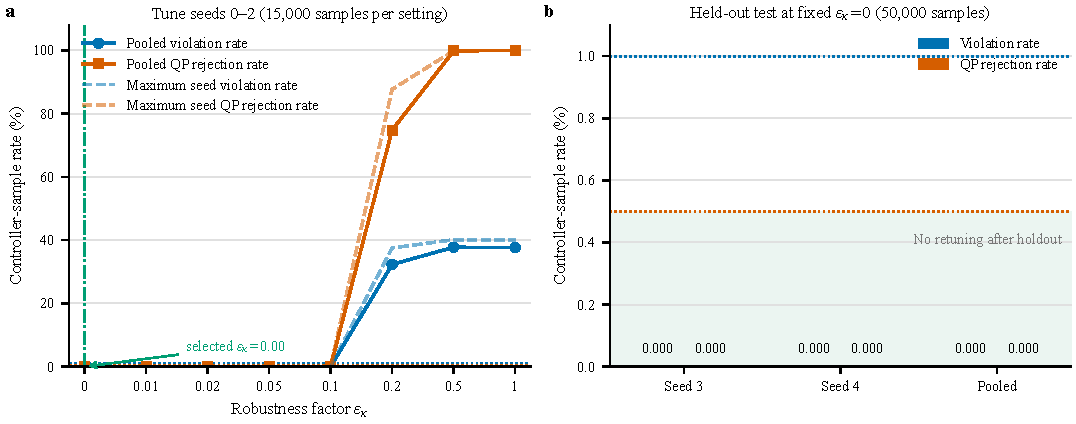
\includegraphics[width=0.95\textwidth]{figures/Figure_2.pdf}
    \caption{Process trajectories under S3: Coupled state-dependent perturbation (PPO-RHOCBF, $\epsilonKappa=1.0$, 500 steps). Top: main steam pressure (bounds: 13--24\,MPa). Middle: separator outlet enthalpy (bounds: 2670--2830\,kJ/kg). Bottom: turbine power output ($\pm$50\,MW of 1000\,MW target). All three variables remain within their constraint bounds throughout the 500-step evaluation.}
    \label{fig:trajectories}
\end{figure*}

\begin{figure}[t]
    \centering
    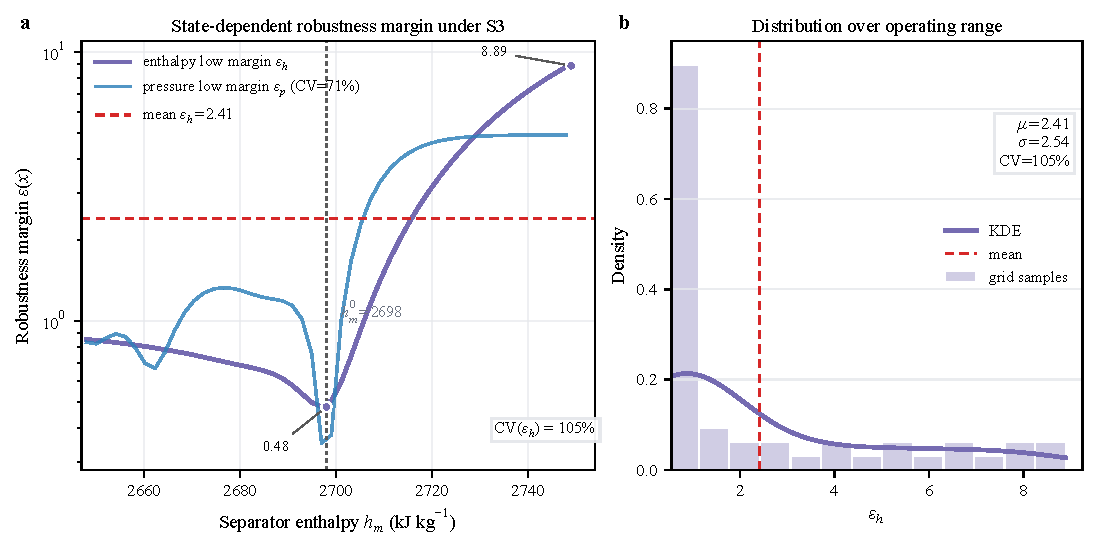
\includegraphics[width=\columnwidth]{figures/Figure_3.pdf}
    \caption{Safety filter behavior under S3: Coupled perturbation (PPO-RHOCBF, $\epsilonKappa=1.0$). Top: compositional robustness margin $\epsilon(x)$ ($\mathrm{CV}=70\%$). Middle: minimum constraint margin (positive = safe). Bottom: QP safety filter intervention.}
    \label{fig:safety_behavior}
\end{figure}

\begin{figure}[t]
    \centering
    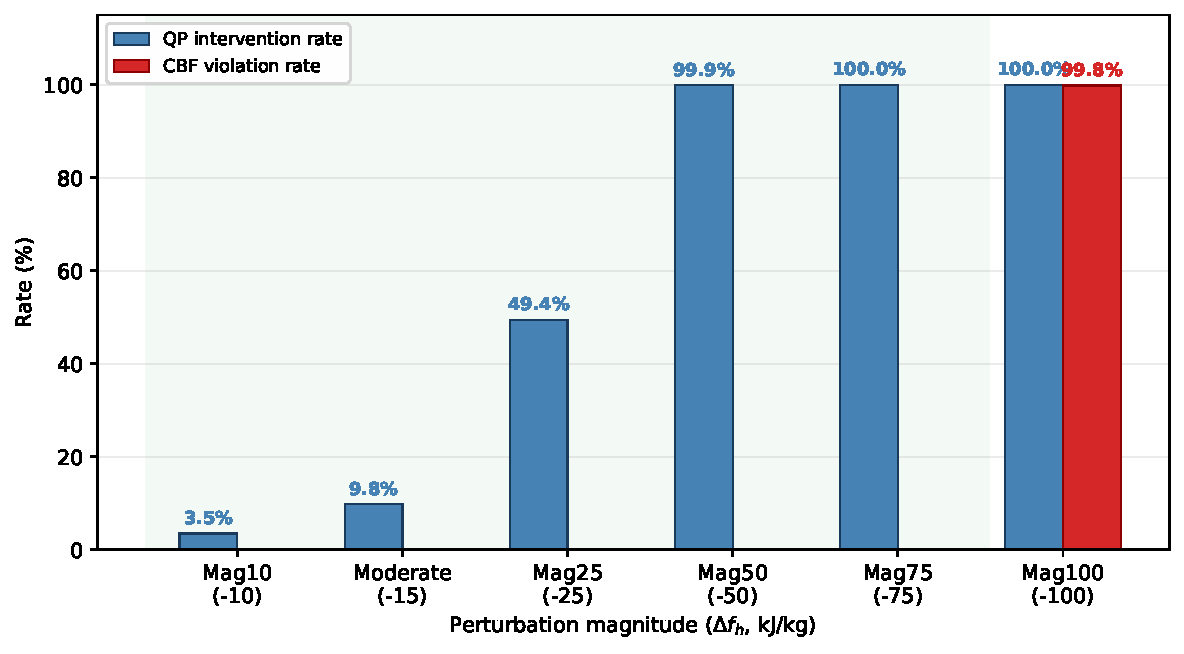
\includegraphics[width=\columnwidth]{figures/Figure_4.pdf}
    \caption{QP intervention rate vs.\ perturbation magnitude (S1:Heat structure, PPO-RHOCBF, 3 seeds).}
    \label{fig:qp_intervention}
\end{figure}

\begin{figure}[t]
    \centering
    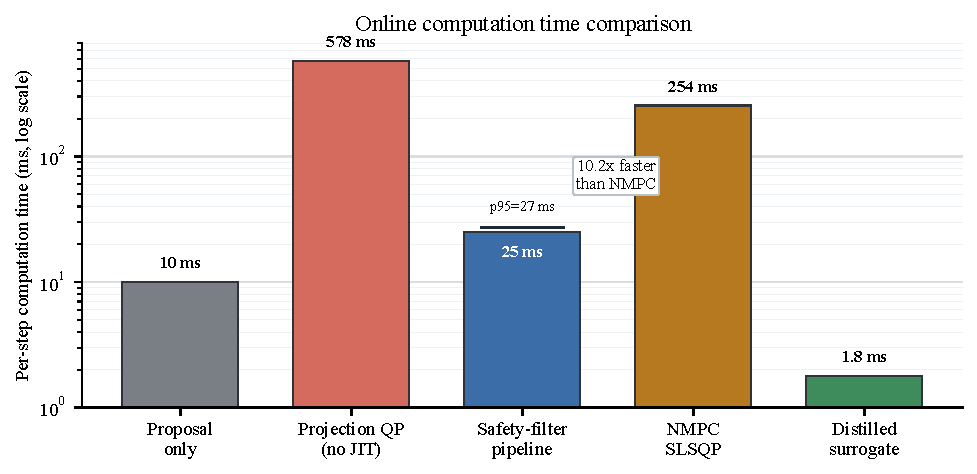
\includegraphics[width=\columnwidth]{figures/Figure_5.pdf}
    \caption{Per-step online computation time (NVIDIA RTX 4090 GPU for RL+QP JIT; AMD Ryzen 9 7950X CPU for NMPC). RL+QP (JIT, incl.\ GP): ${\sim}25$\,ms; PPO only: ${\sim}10$\,ms; PPO+QP (no JIT): ${\sim}578$\,ms; NMPC: 254\,ms; distilled: 1.8\,ms (CPU, empirical-only safety).}
    \label{fig:computation_time}
\end{figure}

The reported ${\sim}25$\,ms per step (JIT-compiled, GPU) includes the PPO forward pass, GP inference, and QP solve; GP inference contributes approximately ${\sim}5$\,ms of this total. NMPC with $N=10$ horizon and SLSQP solver averages 254\,ms per step (CPU). The distilled policy achieves 1.8\,ms inference (CPU) with empirical-only safety. The $10\times$ speedup over NMPC and the per-step (rather than horizon-based) safety evaluation are the key computational advantages for real-time process control deployment.

\subsection{Key Ablation Findings}

Detailed ablation results appear in the Supplementary Material. Key findings: (1)~All $\epsilonKappa \in [0.3, 1.0]$ achieve 0\% CBF violation on S1 and S3; Theorem~1 certifies only $\epsilonKappa = 1$. (2)~$\sigma_{\mathrm{floor}}$-dominated $\epsilon(x)$ under constant perturbations (S1: floor fraction ${\sim}30\%$) vs.\ data-driven $\epsilon(x)$ under state-dependent perturbations (S3: floor fraction $<0.1\%$, $\mathrm{CV}(\epsilon_h)=70\%$). (3)~Scenario-specific GP training is a prerequisite: generic mixed GP achieves 82.7--99.7\% violation under perturbation (Supplementary). (4)~OOD asymmetry: S1$\to$S3 achieves 0\% (large $\sigmaGP$ inflates $\epsilon$), while S3$\to$S1 reaches $99.9\%$ violation ($\sigmaGP$ is small despite biased mean).
